%%%%%%%%%%%%%%%%%%%%%%%%%%%%%%%%%%%%%%%%%%%%%%%%%%%%%%%%%%%%%%%%%%%%%%
%     File: ExtendedAbstract_intro.tex                               %
%     Tex Master: ExtendedAbstract.tex                               %
%%%%%%%%%%%%%%%%%%%%%%%%%%%%%%%%%%%%%%%%%%%%%%%%%%%%%%%%%%%%%%%%%%%%%%

\section{Introduction}
\label{sec:intro}

Referring Instance Segmentation is a fundamental task in computer vision that requires models to identify and segment specific object instances using natural language descriptions. When applied to aerial photographs, also referred to as Referring Remote Sensing Instance Segmentation (RRSIS), this task represents a major challenge due to the intricate characteristics of aerial imagery, including varying scales and resolutions of top-down perspectives, geographic complexities, extreme object density variations, and unique spatial relationships not present in ground-level photography.

\begin{figure}[H]
\centering
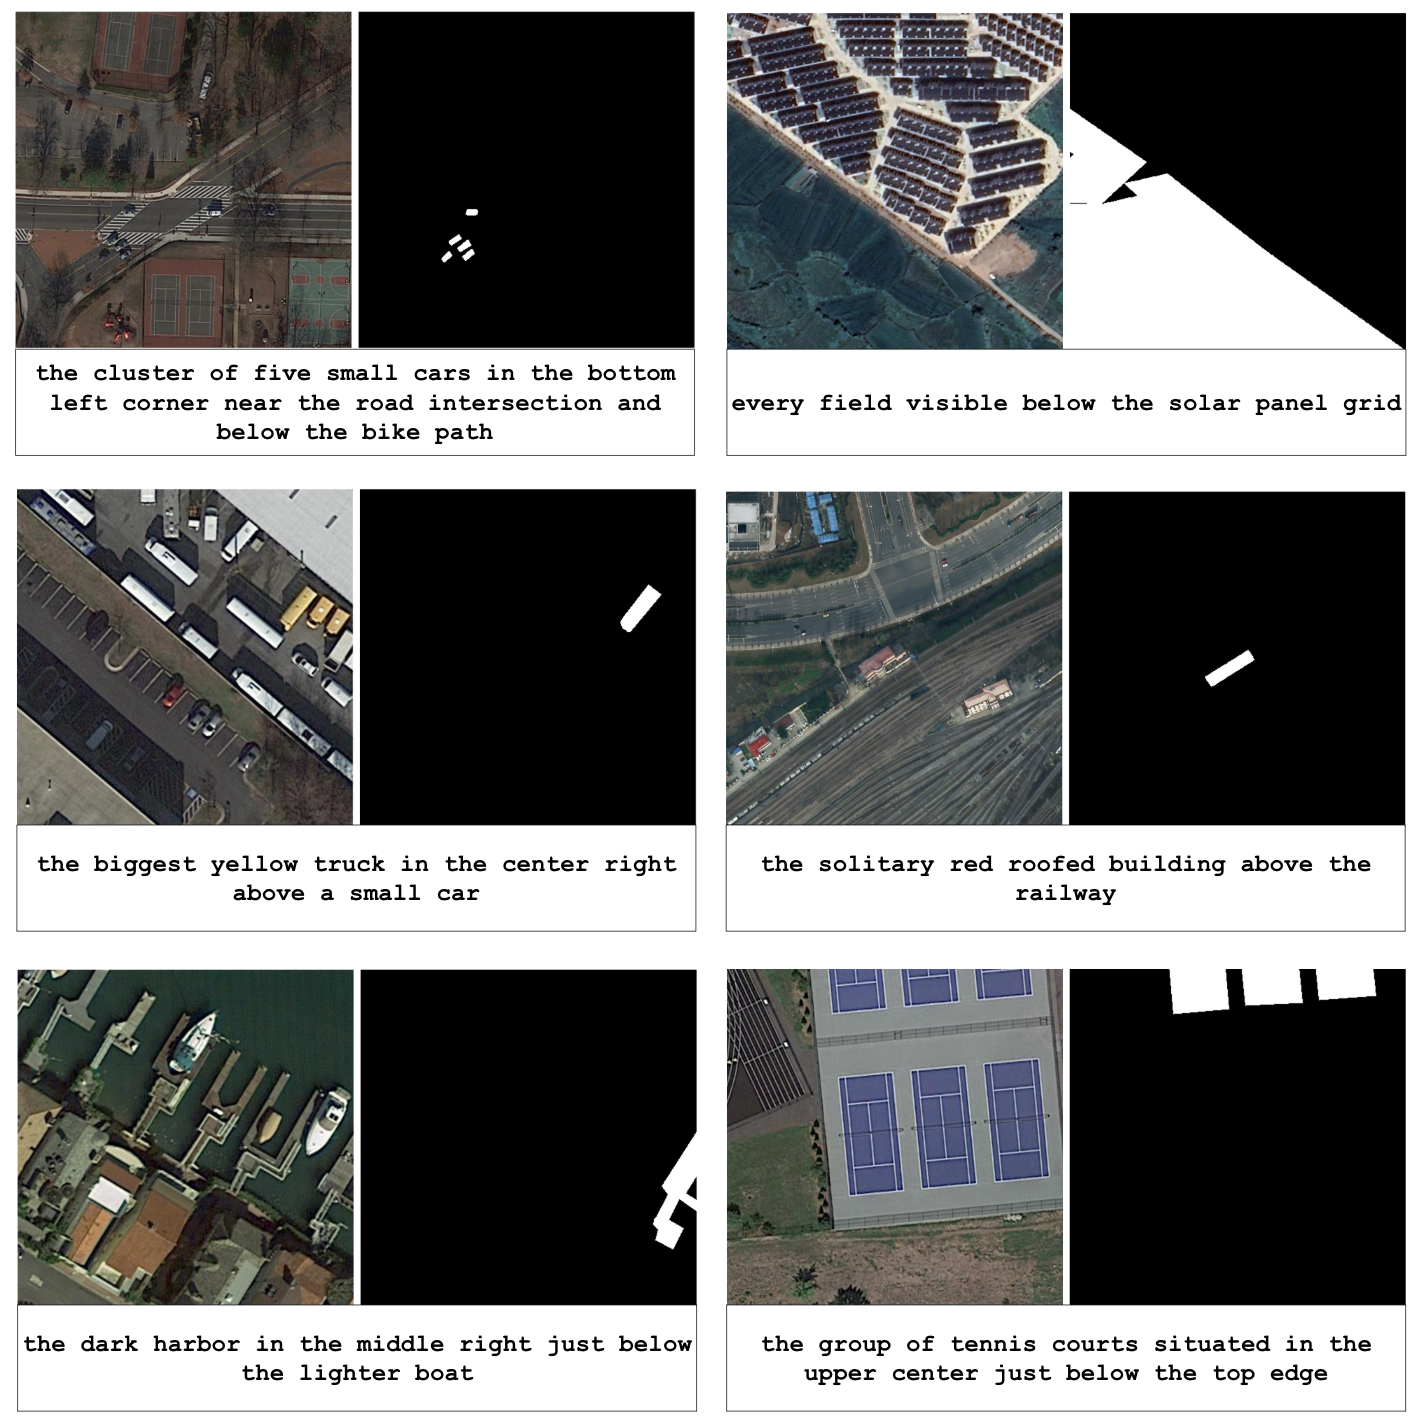
\includegraphics[width=\columnwidth]{./images/6samples.png}
\caption{Representative examples from Aerial-D dataset showing diverse referring expressions with corresponding aerial images and ground truth masks.}
\label{fig:dataset_examples}
\end{figure}

A critical component for developing effective models for RRSIS is access to high-quality datasets containing aerial photographs, precise segmentation masks, and natural referring expressions. To address this need, we introduce Aerial-D, the largest referring segmentation dataset for aerial imagery to date, comprising over 1.5 million expressions across 37,288 aerial image patches. The primary focus of Aerial-D is not only to provide exceptional training data quality but also to establish the most challenging benchmark for RRSIS to date, which will hopefully prompt research into novel RRSIS model architectures that can surpass current performance limitations.

Our key contributions include: (1) We introduce a comprehensive set of tools that enable the production of complex referring expression datasets from instance segmentation datasets, including a rule-based pipeline, novel LLM enhancement and distillation methods, and historic image data augmentation using proposed filters. (2) Using these tools, we construct Aerial-D, a massive dataset comprising over 1.5 million expressions across 37,288 aerial image patches, representing the largest referring segmentation dataset for aerial imagery to date. (3) We present a unified model trained on Aerial-D alongside four additional datasets, applying our tools including historic transformations across all training data. This model demonstrates capabilities for referring instance segmentation, referring group segmentation, class-based segmentation, land cover segmentation, and robust handling of historic imagery including black and white, grainy, or sepia photographs.

